\section{Primary-pair quality and latency}
\label{sec:wins}

\subsection{Quality on the same log events}
The relevant quality comparison is between AR-30B and DG themselves.
We re-score their saved outputs on the same 300 BGL events with the same
nine-field metric and parser-derived references. Table~\ref{tab:primaryquality}
places this comparison beside its generation times.

\begin{table}[ht]
\centering
\caption{Primary pair on 300 shared events. F1 measures extraction agreement;
schema validity checks record structure. These are paired-sample timings,
separate from the larger repeated latency sample.}
\label{tab:primaryquality}
\begin{tabular}{@{}lrr@{}}
\toprule
Measure & AR-30B & DG \\
\midrule
Nine-field F1 & 0.870 & 0.852 \\
Schema-valid records (\%) & 99.3 & 99.0 \\
Paired-sample median (ms) & 924.2 & 373.7 \\
\bottomrule
\end{tabular}

\end{table}

DG's extraction score is close to AR's, and a paired bootstrap analysis
supports a small average DG deficit. The saved outputs therefore show a
faster response with a modest loss on this metric, rather than equal
quality. Whether that tradeoff is acceptable depends on the task;
Appendix~\ref{app:protocol} reports the difference, uncertainty interval,
and scoring limits without choosing an equivalence margin after the fact.

\subsection{Reading a generation-time budget}
For the larger repeated timing sample, median latency is
\dgMedian\,ms for DG and \arMedian\,ms for AR-30B. The median describes
the middle request; a deadline asks a different question: what fraction
has finished by a specified time?

Figure~\ref{fig:distributions} answers that question directly. Pick a time
on the horizontal axis, move up to a model's curve, and read the percentage
of completed generations. At 1,000\,ms, nearly all DG responses have
finished, while about three quarters of AR responses have. A steep section
means many requests finish in a narrow time range.

\begin{figure}[ht!]
\centering
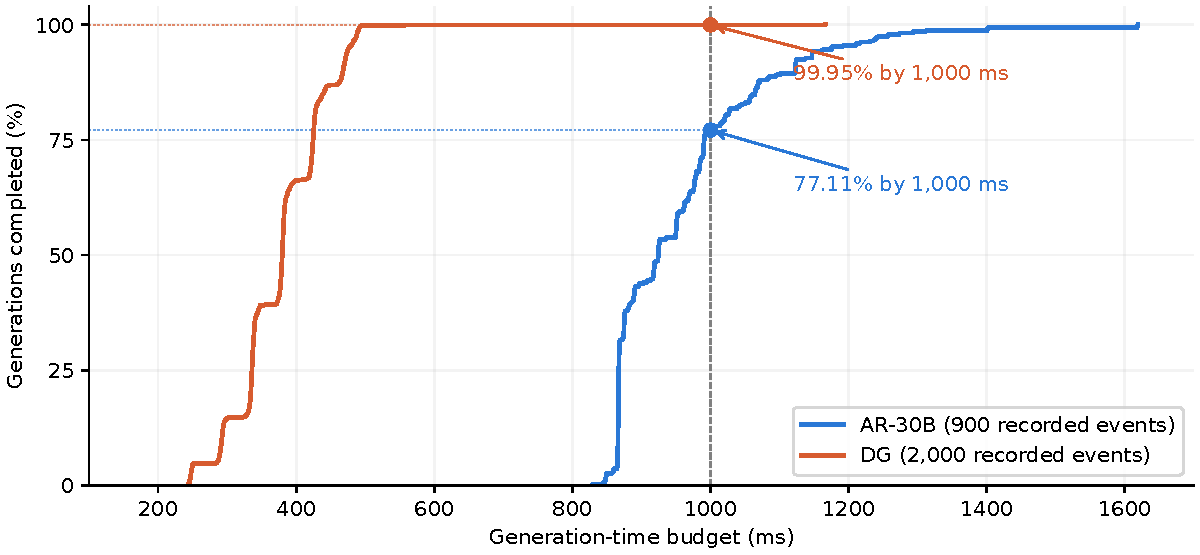
\includegraphics[width=.95\linewidth]{figures/fig12_v8.pdf}
\caption{Percentage of saved generations completed within each time budget
(AR-30B: 900 events across three runs; DG: 2,000 events).
Dots and guides show the 1,000\,ms example. These are generation times,
not end-to-end response times or correctness rates.}
\label{fig:distributions}
\end{figure}

\begin{table}[ht]
\centering
\caption{Generation-budget coverage (\%). Valid also requires the harness
schema check. All recorded events remain in the denominator; semantic
correctness and downstream processing are not assessed here.}
\label{tab:budgets}
\begin{tabular}{@{}rrrrr@{}}
\toprule
& \multicolumn{2}{c}{Completed} & \multicolumn{2}{c}{Valid and completed} \\
Budget (ms) & AR-30B & DG & AR-30B & DG \\
\midrule
500 & 0.00 & 99.80 & 0.00 & 98.50 \\
1000 & 77.11 & 99.95 & 76.44 & 98.65 \\
\bottomrule
\end{tabular}

\end{table}

At a 500\,ms generation budget, DG supplies structurally valid records
for most events and this AR configuration supplies none. This is a
concrete reason to evaluate DG for a time-constrained service, provided its
extraction quality meets the application's needs. It is not a claim that
every possible AR configuration misses the same target.
